\section{附加实验}

\subsection{可视化假设~\labelcref{item:lindeberg-condition} 的分解}

\cref{fig:time} 展示了我们的分析模型在训练过程中足够长的时间内有效,能够捕捉到单个 ReLU 神经元中的定位现象(\labelcref{item:single-neuron-model})。
在前面三列中,我们可视化了来自我们经验模型和分析模型的权重的 IPR,以及这两个权重之间的 $\ell_2$ 差异。
在前四行中,我们可视化了这些指标,分别对应模型的四个随机初始化,每个初始化在 $\texttt{NLGP}(g=100)$ 上训练,且 $\xi_0 = 0.3$ 和 $\xi_1 = 0.7$,根据 \cref{thm:localization},我们期望看到定位现象。
我们看到,在 IPR 增加后不久,误差迅速增加,表明局部感受野的形成。
最后三列确认了这一点,它们展示了在经验权重和分析权重之间的发散发生前、中、后的快照。
我们观察到,权重在 \emph{之前} 几乎完全相同,在 \emph{期间} 最局部化的点仅有微小差异,而在 \emph{之后} 都是局部化的,但可能具有不同的幅度和位置。
在 \emph{期间} 出现的差异是由于假设~\labelcref{item:lindeberg-condition} 的失效,这个假设在构建我们的分析模型时使用,当 $\mathbf{w}$ 的范数被少数几项主导时(即局部化时)会被违背。
虽然 \cite{ingrosso2022data} 也观察到他们的分析模型在局部化出现时发生崩溃,但我们的方法关键地在足够长的时间内有效,从而能够表征局部化的出现。

我们将对各个子图进行更详细的讨论。
在 \cref{fig:time} 的所有行中,除了第三行,分析预测几乎完全准确;在第三行中,我们预测了定位现象,但位置错误。
再次聚焦在第一行,我们看到在 $t=20$ 时,权重尚未局部化(从 IPR 左侧、第一列和视觉上来看),分析权重和经验权重几乎完全一致,这一点可以通过左侧、中心上方的小距离确认。
在 $t=30$ 时,围绕 $i=21$ 的局部峰值开始出现,这违背了假设 \labelcref{item:lindeberg-condition},并削弱了分析精度。
分析模型低估了主峰 $i=21$ 的主导程度,同时高估了 $i=30$、$37$ 和 $90$ 处竞争峰的大小。
尽管如此,在 $t=50$ 时,我们看到分析模型的预测仍然与经验模型相匹配。

在 \cref{fig:time} 的最后一行,我们使用与第一行相同的初始化和设置,只不过我们改为在 $\texttt{NLGP}(g=0.01)$ 数据上进行训练。
根据 \cref{thm:localization},我们\emph{不}期望看到定位现象。
IPR 的演化确认了这一点,因为它保持在较低的幅度。
我们还观察到,由于定位现象从未出现,假设~\labelcref{item:lindeberg-condition} 从未被违背,因此我们的分析模型几乎完全符合经验模型。

\newcommand{\sampleheight}{42pt}
\newcommand{\covheight}{46pt}
\newcommand{\marginalheight}{50pt}
\setlength{\tabcolsep}{4pt}
\begin{figure}[t]
  \centering
  \hspace{-1.2em}
  \scalebox{0.9}{
  \begin{centering}
    \begin{tabular}{p{51pt}
      @{\hspace{10pt}}m{2pt}l
      @{\hspace{5pt}}l
      @{\hspace{10pt}}m{2pt}l
      @{\hspace{10pt}}m{2pt}l}
        \raisebox{18pt}{\small$\texttt{Ising}$} &
        \raisebox{34pt}{\rotatebox{90}{\tiny input value}} &
        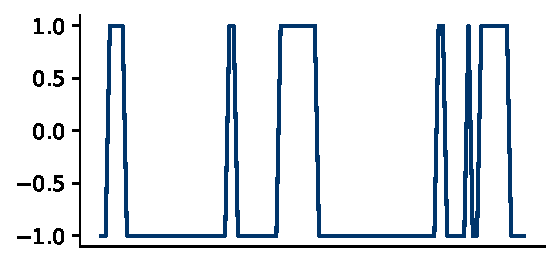
\includegraphics[height=\sampleheight]{figures/task/samples_long/ising.pdf} &
        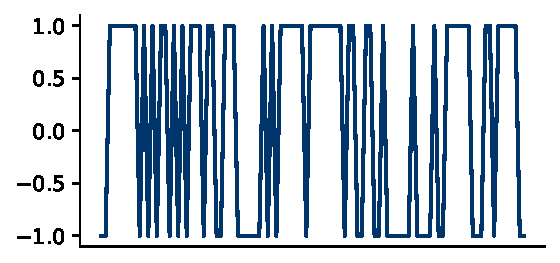
\includegraphics[height=\sampleheight]{figures/task/samples_short/ising.pdf} &
        \raisebox{38pt}{\rotatebox{90}{\tiny input dimension}} &
        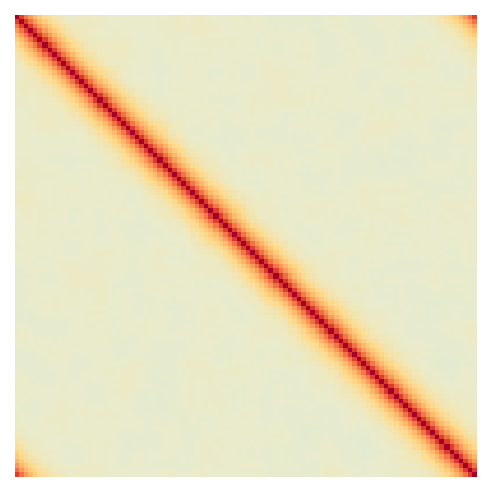
\includegraphics[height=\covheight]{figures/task/cov/ising.pdf} &
        \raisebox{40pt}{\rotatebox{90}{\tiny $p(X_i)$}} &
        \raisebox{-4pt}{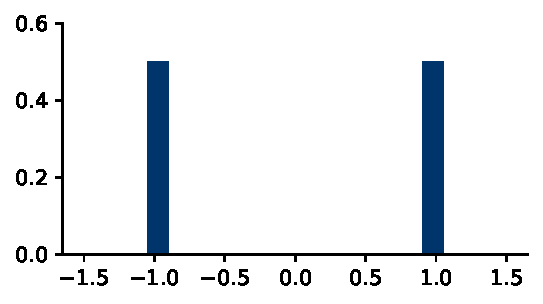
\includegraphics[height=\marginalheight]{figures/task/marginal/ising.pdf}} \\
        \noalign{\vskip -36pt}
        \raisebox{18pt}{\small$\texttt{NLGP}(0.01)$} &
        \raisebox{34pt}{\rotatebox{90}{\tiny input value}} &
        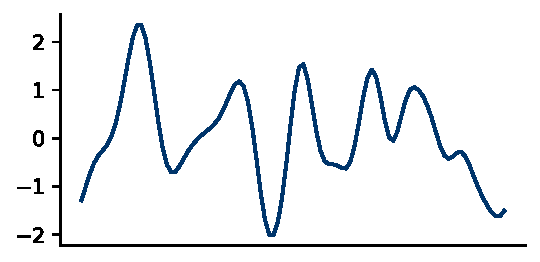
\includegraphics[height=\sampleheight]{figures/task/samples_long/gaussian.pdf} &
        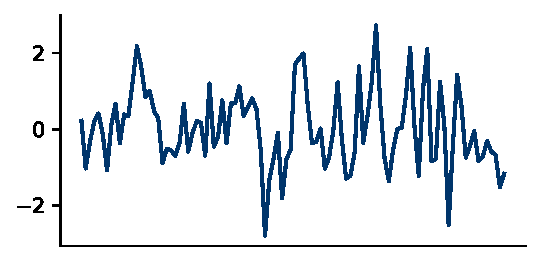
\includegraphics[height=\sampleheight]{figures/task/samples_short/gaussian.pdf} &
        \raisebox{38pt}{\rotatebox{90}{\tiny input dimension}} &
        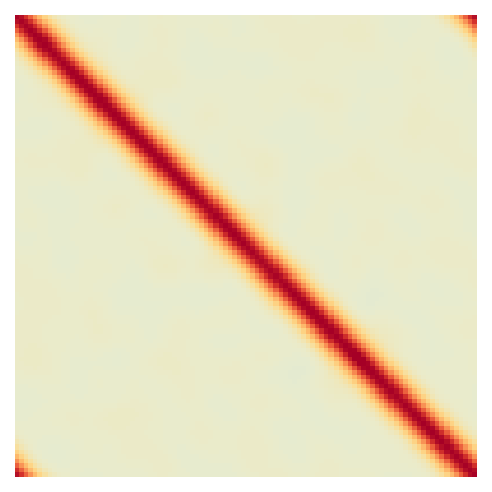
\includegraphics[height=\covheight]{figures/task/cov/gaussian.pdf} &
        \raisebox{40pt}{\rotatebox{90}{\tiny $p(X_i)$}} &
        \raisebox{-4pt}{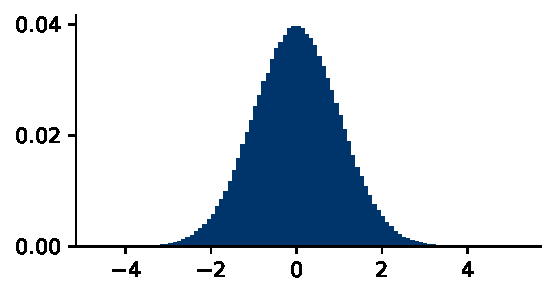
\includegraphics[height=\marginalheight]{figures/task/marginal/gaussian.pdf}} \\
        \noalign{\vskip -36pt}
        \raisebox{18pt}{\small $\texttt{Kur}(5)$} &
        \raisebox{34pt}{\rotatebox{90}{\tiny input value}} &
        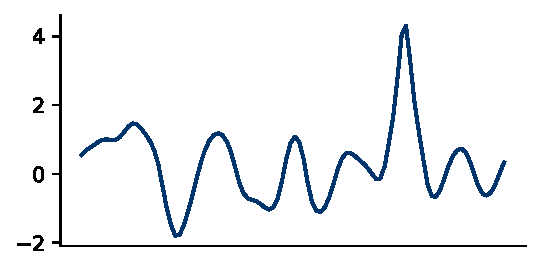
\includegraphics[height=\sampleheight]{figures/task/samples_long/alg5.pdf} &
        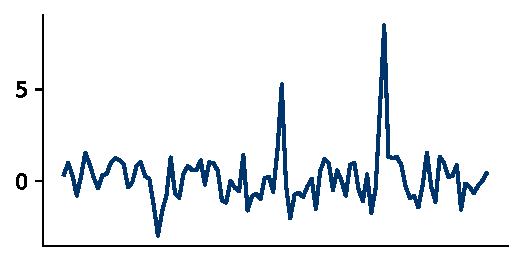
\includegraphics[height=\sampleheight]{figures/task/samples_short/alg5.pdf} &
        \raisebox{38pt}{\rotatebox{90}{\tiny input dimension}} &
        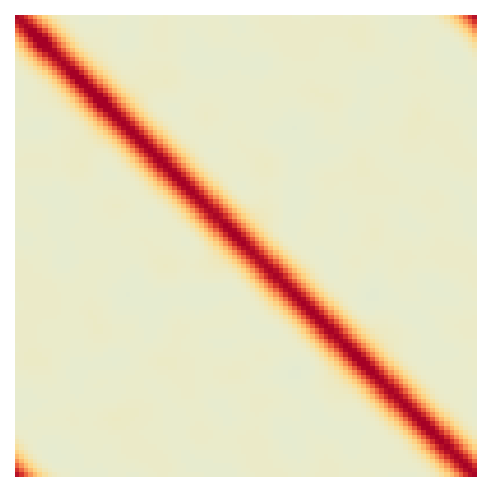
\includegraphics[height=\covheight]{figures/task/cov/alg5.pdf} &
        \raisebox{40pt}{\rotatebox{90}{\tiny $p(X_i)$}} &
        \raisebox{-4pt}{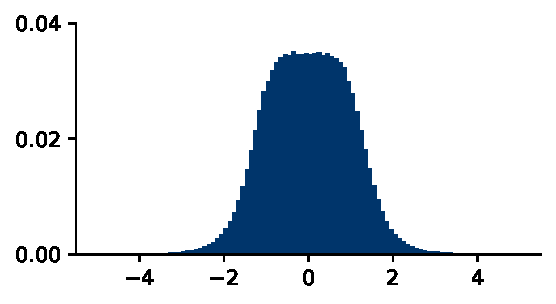
\includegraphics[height=\marginalheight]{figures/task/marginal/alg5.pdf}} \\
        \noalign{\vskip -37pt}
        &&
        \hspace{25pt}\tiny input dimension &
        \hspace{25pt}\tiny input dimension & &
        \hspace{3pt}\tiny input dimension & &
        \hspace{37pt}\tiny input value \\
  \end{tabular}
  \end{centering}
  }
  \caption{
    从左到右:
    长尺度和短尺度样本 $\mathbf{x}$,
    单一尺度的协方差 $\Sigma$,
    以及数据模型的边缘分布 $p(X_i)$,如 \cref{sec:task} 所述:
    Ising 模型(左、右样本分别为 $J=1.2, 0.3$),
    非线性高斯过程~\parencite[NLGP;~][]{ingrosso2022data},
    以及可控峰度模型 \texttt{Kur}
    (左、右样本分别为 $\xi=5, 1$)。
    \emph{
    每个模型生成的样本以零为中心,且其协方差可以被约束为相似,
    但具有不同的高阶统计量,从维度方向的边缘分布中可以看出这一点。
    }
}
  \label{fig:task}
  \vspace{-10pt}
\end{figure}

